\documentclass[a4paper]{scrartcl}
\usepackage[cm]{fullpage}
\usepackage{amsmath, amssymb}

\usepackage{sectsty}
\sectionfont{\large\selectfont}
\subsectionfont{\normalsize\selectfont}

\usepackage{siunitx}
\usepackage{tikz}

\begin{document}

\title{PHYS1241: Assignment 2}
\author{ \\ \\ }
\date{2015-09-09}
\maketitle

\section{In a certain region of space, there is a uniform electric field \(\mathbf{E}\) of \SI{10000}{\volt\per\centi\metre} in the \(+x\) direction. In the same region of space there is a uniform magnetic field \(\mathbf{B}\) in the \(+y\) direction. A beam of mu-mesons with velocity \(\frac{c}{3}\) travels through this region in a straight line in the \(+z\) direction.}
\subsection{What is the strength of the field \(\mathbf{B}\)?}
Since the charges are travelling in a straight line with constant velocity, there must be no net force acting on them, and this can be used to calculate the magnetic field:
\begin{align*}
    \mathbf{E} &= \begin{pmatrix}\mathbf{E}_x \\ 0 \\ 0\end{pmatrix},
    \mathbf{B} = \begin{pmatrix}0 \\ \mathbf{B}_y \\ 0\end{pmatrix},
    \mathbf{v} = \begin{pmatrix}0 \\ 0 \\ \mathbf{v}_z\end{pmatrix} \\
    \mathbf{F} &= q (\mathbf{E} + \mathbf{v} \times \mathbf{B}) = \mathbf{0} \\
    &= q \begin{pmatrix}\mathbf{E}_x - \mathbf{v}_z \mathbf{B}_y \\ 0 \\ 0\end{pmatrix} \\
    \therefore \mathbf{E}_x &= \mathbf{v}_z \mathbf{B}_y \\
    \mathbf{B}_y &= |\mathbf{B}| = \frac{\mathbf{E}_x}{\mathbf{v}_z} \\
    &= \frac{\SI{30000}{\volt\per\centi\metre}}{c} \approx \SI{10}{\milli\tesla}
\end{align*}

\subsection{Can you tell from this experiment if the charge on the meson is positive or negative?}
No, since the \(q\) term in the equation turns out to be irrelevant.

Physically, a positive charge would be attracted to the \(+x\) direction by the \(\mathbf{E}\)-field, and to the \(-x\) direction by the \(\mathbf{B}\)-field, and the exact opposite would happen for a negative charge. But since the charge travels in a straight line, that is, experiencing no net force, the two fields balance each other perfectly so it is impossible to determine whether the charge is attracted to \(+x\) or \(-x\) by the \(\mathbf{E}\)- or \(\mathbf{B}\)-field, and thus impossible to determine the sign of the charge.

\section{A metal spherical shell of inner radius \(a\) and outer radius \(b\) is located with its centre at the origin. There is a small hole cut at one point of the shell.}
\subsection{If there is no net charge on the shell, how much work is required to bring a charge \(q_1\) from infinity, through the hole and to the origin?}
No work is required, as the uncharged shell does not generate any electric potential.

\subsection{How much work is required if the shell is given a total charge \(q_2\)?}
Find the electric potential at the centre of the charged shell, and then multiply it by \(q_1\) to determine the work required. Since a charged conductor will have the charges distributed only over its outer surface, we only need to consider the sphere as if it were a infinitesimally thin sphere at \(r = b\).
\begin{align*}
    V_E &= \iint_S \frac{\mathrm{d}q_2}{4 \pi \varepsilon_0 r} \\
    &= \int_0^\pi \int_0^{2 \pi} \frac{\sigma}{4 \pi \varepsilon_0 r} r^2 \sin \phi \,\mathrm{d}\theta \,\mathrm{d}\phi \\
    \sigma &= \frac{q_2}{4 \pi r^2} \\
    V_E &= \frac{q_2}{(4 \pi)^2 \varepsilon_0 r} \int_0^\pi \int_0^{2 \pi} \sin \phi \,\mathrm{d}\theta \,\mathrm{d}\phi \\
    &= \frac{q_2}{4 \pi \varepsilon_0 r} \\
    \therefore U_E \bigg|_{r = b} &= q_1 V_E \bigg|_{r = b} \\
    &= \frac{q_1 q_2}{4 \pi \varepsilon_0 b}
\end{align*}

\section{A parallel plate capacitor is connected to a battery that maintains a potential difference \(V_0\) between its plates. A slab of dielectric constant \(\kappa\) is inserted between the plates, completely filling the space between them.}
\subsection{Show that the battery does an amount of work \(q_0 V_0 (\kappa - 1)\) during the insertion process, if \(q_0\) is the charge on the capacitor before the slab is inserted.}
The work done by a constant voltage source (the battery in this case) is just the amount of charge moved multiplied by the voltage:
\begin{align*}
    W &= V_0 \Delta q = V_0 (q_1 - q_0) \\
    q_0 &= C_0 V_0 \\
    q_1 &= \kappa C_0 V_0 = \kappa q_0 \\
    \therefore W &= q_0 V_0 (\kappa - 1)
\end{align*}

\subsection{How much work is done by mechanical forces on the slab when it is inserted between the plates? Is this work done on, or by, the agent inserting the slab?}
The net amount of energy added to the capacitor is:
\begin{align*}
    \Delta E &= \frac{1}{2} \kappa C_0 V_0^2 - \frac{1}{2} C_0 V_0^2 \\
    &= \frac{1}{2} q_0 V_0 (\kappa - 1)
\end{align*}

Since only half the work done by the battery became energy stored in the capacitor, the remaining work must have been done to the dielectric, pulling it inside the capacitor, assuming no resistive or radiative losses.

Thus the work done \emph{on} the dielectric, towards the capacitor, is:
\[W - \Delta E = \frac{1}{2} q_0 V_0 (\kappa - 1)\]

\section{A wire bent is into the shape shown. A current \(I = \SI{15}{\ampere}\) flows through the wire, \(a\) has length \SI{5.2}{\centi\metre}. What is the magnetic field \(\mathbf{B_P}\) at point \(P\)?}
\begin{center}
    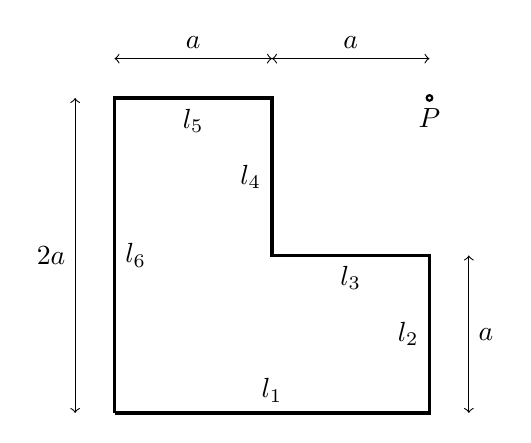
\begin{tikzpicture}
        \draw [very thick]
            (0, 0) -- (4, 0) node[midway, above] {\(l_1\)}
            -- (4, 2) node[midway, left] {\(l_2\)}
            -- (2, 2) node[midway, below] {\(l_3\)}
            -- (2, 4) node[midway, left] {\(l_4\)}
            -- (0, 4) node[midway, below] {\(l_5\)}
            -- (0, 0) node[midway, right] {\(l_6\)};
        \draw [thick] (4, 4) circle (1 pt) node [below] {\(P\)};
        \draw [<->] (-0.5, 0) -- (-0.5, 4) node [midway, left] {\(2 a\)};
        \draw [<->] (0, 4.5) -- (2, 4.5) node [midway, above] {\(a\)};
        \draw [<->] (2, 4.5) -- (4, 4.5) node [midway, above] {\(a\)};
        \draw [<->] (4.5, 2) -- (4.5, 0) node [midway, right] {\(a\)};
    \end{tikzpicture}
\end{center}
We can use the Biot-Savart law to find the magnetic field due to a wire segment, and then apply it to each segment of the wire loop.

For a wire segment on the \(+x\) axis starting at the origin and of length \(l\), and constant current \(I\) flowing away from the origin, the magnetic field can be derived for any arbitrary 2D displacement:
\begin{align*}
    \mathbf{B}(\mathbf{r}) &= \frac{\mu_0 I}{4 \pi} \int_C \frac{\mathrm{d}\mathbf{l} \times \mathbf{r}'}{|\mathbf{r}'|^3} \\
    \mathbf{r} &= \begin{pmatrix}x \\ y \\ 0\end{pmatrix}, \mathbf{l} = \begin{pmatrix}l \\ 0 \\ 0\end{pmatrix} \\
    \mathbf{r}' &= \mathbf{r} - \mathbf{l} = \begin{pmatrix}x - l \\ y \\ 0\end{pmatrix} \\
    \mathrm{d}\mathbf{l} \times \mathbf{r}' &= \begin{pmatrix}0 \\ 0 \\ y \,\mathrm{d}l\end{pmatrix} \\
    \therefore \mathbf{B}(\mathbf{r}) &= \frac{\mu_0 I}{4 \pi} \begin{pmatrix}
        0 \\ 0 \\
        \int_0^l \frac{y \,\mathrm{d}l}{((x - l)^2 + y^2)^{\frac{3}{2}}}
    \end{pmatrix} \\
    \therefore \mathbf{B}_z(\mathbf{r}) &= \begin{cases}
        0 & y = 0 \\
        \frac{\mu_0 I}{4 \pi y} \left( \frac{l - x}{\sqrt{(l - x)^2 + y^2}} + \frac{x}{\sqrt{x^2 + y^2}} \right) & \text{Otherwise}
    \end{cases}
\end{align*}

Now consider going anticlockwise around the wire loop starting at wire segment \(l_1\), placing the origin of each wire segment at the start of each and the \(+x\) axis along the wire. This can be done because \(\mathbf{B}(\mathbf{r})\) is independent of the \(x\) and \(y\) axis. \(\mathbf{B_P}\) can then be calculated:
\begin{align*}
    \mathbf{B_P}_z &=
    \mathbf{B}_z\begin{pmatrix}2 a \\ 2 a \\ 0\end{pmatrix} \bigg|_{l = 2 a} +
    \mathbf{B}_z\begin{pmatrix}2 a \\ 0 \\ 0\end{pmatrix} \bigg|_{l = a} +
    \mathbf{B}_z\begin{pmatrix}0 \\ -a \\ 0\end{pmatrix} \bigg|_{l = a} \\
    &+ \mathbf{B}_z\begin{pmatrix}a \\ -a \\ 0\end{pmatrix} \bigg|_{l = a} +
    \mathbf{B}_z\begin{pmatrix}-a \\ 0 \\ 0\end{pmatrix} \bigg|_{l = a} +
    \mathbf{B}_z\begin{pmatrix}0 \\ 2 a \\ 0\end{pmatrix} \bigg|_{l = 2 a} \\
    &= \frac{-\mu_0 I}{4 \pi a \sqrt{2}} \\
    \therefore \mathbf{B_P} &= \begin{pmatrix}0 \\ 0 \\ \frac{-\mu_0 I}{4 \pi a \sqrt{2}}\end{pmatrix} \approx \begin{pmatrix}0 \\ 0 \\ -20\end{pmatrix}\si{\micro\tesla}
\end{align*}
Where \(I\) is assumed to be flowing anticlockwise. If it were flowing clockwise, the sign would just be reversed. In other words, an anticlockwise current would cause \(\mathbf{B_P}\) to be in to the page, while a clockwise would be out of the page.

\section{A very long conducting rod of radius \(a\) has an off-centre hole of radius \(b\) whose axis is parallel to but offset by a distance \(d\) from the axis of the rod. A uniform current density \(+j\) flows in the conductor. What is the magnetic field \(\mathbf{B}\) at the axis of the hole, far from the ends?}
Consider the superposition of a radius \(a\) cylinder with current density \(j\) and a radius \(b\) cylinder with current density \(-j\). This is equivalent to the question's setup. Since the magnetic field at the axis of a uniformly conducting cylinder is zero, the radius \(b\) cylinder does not contribute to \(\mathbf{B}\), so we only need to consider the radius \(a\) cylinder at radius \(d\). It can be calculated by taking a circular Amperian loop of radius \(d\) centred on the cylinder axis:
\begin{align*}
    \oint_C \mathbf{B} \cdot \,\mathrm{d}\mathbf{s} &= \mu_0 I_{enc} \\
    |\mathbf{B}| 2 \pi d &= j \pi \mu_0 d^2 \\
    \therefore |\mathbf{B}| &= \frac{j \mu_0 d}{2}
\end{align*}

\pagebreak
\section{Consider two coaxial loops of radius \(a\) which are separated by a distance \(d; d \gg a\). A current \(I = K_0 t^2\) is sent through loop (1). The resistance of the other loop is \(R\).}
\subsection{Neglecting self-inductance, what is the torque, \(\boldsymbol{\tau}\), on loop (2)?}
First, obtain an expression for the \(\mathbf{B}\)-field due to loop (1) along its axis using the Biot-Savart law:
\begin{align*}
    \text{let } z &= d, r = a \\
    \mathbf{B} &= \frac{\mu_0 I}{4 \pi} \int_C \frac{\mathrm{d}\mathbf{l} \times \mathbf{r}'}{|\mathbf{r}'|^3} \\
    \mathbf{r} &= \begin{pmatrix}
        0 \\
        0 \\
        z
    \end{pmatrix}, \mathbf{l} = \begin{pmatrix}
        r \cos \theta \\
        r \sin \theta \\
        0
    \end{pmatrix} \\
    \mathbf{r}' &= \mathbf{r} - \mathbf{l} = \begin{pmatrix}
        -r \cos \theta \\
        -r \sin \theta \\
        z
    \end{pmatrix} \\
    \mathrm{d}\mathbf{l} &= \begin{pmatrix}
        -r \sin \theta \,\mathrm{d}\theta \\
        r \cos \theta \,\mathrm{d}\theta \\
        0
    \end{pmatrix} \\
    \mathrm{d}\mathbf{l} \times \mathbf{r}' &= \begin{pmatrix}
        r z \cos \theta \,\mathrm{d}\theta \\
        r z \sin \theta \,\mathrm{d}\theta \\
        r^2 \,\mathrm{d}\theta
    \end{pmatrix} \\
    \therefore \mathbf{B} &= \frac{\mu_0 I}{4 \pi} \begin{pmatrix}
        \int_0^{2 \pi} \frac{r z \cos \theta}{(r^2 + z^2)^{\frac{3}{2}}} \mathrm{d}\theta \\
        \int_0^{2 \pi} \frac{r z \sin \theta}{(r^2 + z^2)^{\frac{3}{2}}} \mathrm{d}\theta \\
        \int_0^{2 \pi} \frac{r^2}{(r^2 + z^2)^{\frac{3}{2}}} \mathrm{d}\theta
    \end{pmatrix} \\
    &= \frac{\mu_0 I}{4 \pi} \begin{pmatrix}
        0 \\
        0 \\
        \frac{r^2}{(r^2 + z^2)^{\frac{3}{2}}} 2 \pi
    \end{pmatrix} \\
    \therefore \mathbf{B}_z &= \frac{\mu_0 r^2 I}{2 (r^2 + z^2)^{\frac{3}{2}}} \\
    &= \frac{\mu_0 a^2 I}{2 d^3} \text{ (\(d \gg a\))}
\end{align*}

Since \(a \ll d\), the magnetic field in loop (2) is approximated by this axial magnetic field due to loop (1). This can then be used to calculate the magnetic moment on the loop, and thus its torque:
\begin{align*}
    \mathbf{B}_z &= \frac{\mu_0 a^2 K_0 t^2}{2 d^3} \\
    \Phi_B &= \mathbf{B} \cdot \mathbf{S} = \mathbf{B}_z \pi a^2 \\
    &= \frac{\mu_0 \pi a^4 K_0 t^2}{2 d^3} \\
    V &= -\frac{\mathrm{d}\Phi_B}{\mathrm{d}t} = -\frac{\mu_0 \pi a^4 K_0 t}{d^3} \\
    I_2 &= \frac{V}{R} = -\frac{\mu_0 \pi a^4 K_0 t}{R d^3} \text{ (i.e., Opposite to loop (1))} \\
    \boldsymbol{\mu} &= I_2 \mathbf{S} = -\frac{\mu_0 \pi a^4 K_0 t}{R d^3} \pi a^2 \hat{\mathbf{z}} = -\frac{\mu_0 \pi^2 a^6 K_0 t}{R d^3} \hat{\mathbf{z}} \\
    \therefore \boldsymbol{\tau} &= \boldsymbol{\mu} \times \mathbf{B} \\
    &= \mathbf{0}
\end{align*}

\subsection{Show that, if the self inductance is neglected, the force on loop (2) is \(K = \frac{24 \pi^4 a^8 K_0^2 t^3}{(4 \pi \varepsilon_0 c^2)^2 d^7 R}\).}
From the magnetic moment obtained above, the force can be easily calculated:
\begin{align*}
    \mathbf{F} &= \nabla (\boldsymbol{\mu} \cdot \mathbf{B}) \\
    &= \begin{pmatrix}
        \boldsymbol{\mu}_x \frac{\partial \mathbf{B}_x}{\partial x} \\
        \boldsymbol{\mu}_y \frac{\partial \mathbf{B}_y}{\partial y} \\
        \boldsymbol{\mu}_z \frac{\partial \mathbf{B}_z}{\partial z}
    \end{pmatrix} \\
    &= \begin{pmatrix}
        0 \\
        0 \\
        -\frac{\mu_0 \pi^2 a^6 K_0 t}{R d^3} \frac{\mathrm{\partial}}{\partial d} \left( \frac{\mu_0 a^2 K_0 t^2}{2 d^3} \right)
    \end{pmatrix} \\
    \therefore \mathbf{F}_z &= \frac{3 \mu_0^2 \pi^2 a^8 K_0^2 t^3}{2 d^7 R} = \frac{24 \mu_0^2 \pi^4 a^8 K_0^2 t^3}{(4 \pi)^2 d^7 R} \\
    c^2 &= \frac{1}{\mu_0 \varepsilon_0} \leftrightarrow \mu_0 = \frac{1}{\varepsilon_0 c^2} \\
    \therefore \mathbf{F}_z &= \frac{24 \pi^4 a^8 K_0^2 t^3}{(4 \pi \varepsilon_0 c^2)^2 d^7 R}
\end{align*}

\subsection{In what direction is the force?}
Away from loop (1), since Lenz's law states the induced magnetic field opposes the inducing magnetic field. The result derived in (6.2) agrees with this, with the term controlling the direction of the inducing current, and thus magnetic field, \(K_0\), squared, so will always result in a positive force away from loop (1).

\subsection{In what way (quantitatively) is the true force and torque different from your estimate; i.e., how does self-inductance affect the torque and force?}
Let the self-inductance of loop (1) be \(L_1\), and its resistance be \(R_1\). Then the current including the self-inductance \(I_1 = I - I_i\) can be calculated:
\begin{align*}
    I_i &= \frac{V_i}{R_1} = \frac{L_1}{R_1} \frac{\mathrm{d}I}{\mathrm{d}t} \\
    &= \frac{2 L_1 K_0 t}{R_1} \\
    \therefore I_1 &= K_0 t^2 - \frac{2 L_1 K_0 t}{R_1} = K_0 t^2 \left( 1 - \frac{2 L_1}{R_1 t} \right)
\end{align*}

Replacing the above equations' \(I\) with \(I_1\), we can get a new value for the magnetic moment in loop (2) \(\boldsymbol{\mu}\):
\begin{align*}
    \mathbf{B}_z &= \frac{\mu_0 a^2 K_0 t^2}{2 d^3} \left( 1 - \frac{2 L_1}{R_1 t} \right) \\
    \Phi_B &= \mathbf{B} \cdot \mathbf{S} = \mathbf{B}_z \pi a^2 \\
    &= \frac{\mu_0 \pi a^4 K_0 t^2}{2 d^3} \left( 1 - \frac{2 L_1}{R_1 t} \right) \\
    V &= -\frac{\mathrm{d}\Phi_B}{\mathrm{d}t} = -\frac{\mu_0 \pi a^4 K_0 t}{d^3} \left( 1 - \frac{L_1}{R_1 t} \right) \\
    I_2 &= \frac{V}{R} = -\frac{\mu_0 \pi a^4 K_0 t}{R d^3} \left( 1 - \frac{L_1}{R_1 t} \right) \\
    \boldsymbol{\mu} &= I_2 \mathbf{S} = -\frac{\mu_0 \pi a^4 K_0 t}{R d^3} \left( 1 - \frac{L_1}{R_1 t} \right) \pi a^2 \hat{\mathbf{z}} \\
    &= -\frac{\mu_0 \pi^2 a^6 K_0 t}{R d^3} \left( 1 - \frac{L_1}{R_1 t} \right) \hat{\mathbf{z}}
\end{align*}

Since the direction of the magnetic moment is still parallel to the magnetic field, there is still no torque. i.e., \(\boldsymbol{\tau} = \mathbf{0}\). The new force, however, is:
\begin{align*}
    \mathbf{F} &= \nabla (\boldsymbol{\mu} \cdot \mathbf{B}) \\
    &= \begin{pmatrix}
        0 \\
        0 \\
        -\frac{\mu_0 \pi^2 a^6 K_0 t}{R d^3} \left( 1 - \frac{L_1}{R_1 t} \right) \frac{\partial}{\partial d} \left( \frac{\mu_0 a^2 K_0 t^2}{2 d^3} \left( 1 - \frac{2 L_1}{R_1 t} \right) \right)
    \end{pmatrix} \\
    \therefore \mathbf{F}_z &= \frac{3 \mu_0^2 \pi^2 a^8 K_0^2 t^3}{2 d^7 R} \left( 1 - \frac{L_1}{R_1 t} \right) \left( 1 - \frac{2 L_1}{R_1 t} \right) \\
    &= \frac{24 \pi^4 a^8 K_0^2 t^3}{(4 \pi \varepsilon_0 c^2)^2 d^7 R} \left( 1 - \frac{L_1}{R_1 t} \right) \left( 1 - \frac{2 L_1}{R_1 t} \right)
\end{align*}

Thus, when self-induction is taken into account, the force on loop (2) is multiplied by \(k = \left( 1 - \frac{L_1}{R_1 t} \right) \left( 1 - \frac{2 L_1}{R_1 t} \right)\). This equation goes through the following changes:
\begin{align}
    k > 1 &\text{ when } t < \frac{2 L_1}{3 R_1} \\
    0 \leq k \leq 1 &\text{ when } \frac{2 L_1}{3 R_1} \leq t \leq \frac{L_1}{R_1} \\
    -\frac{1}{8} \leq k < 0 &\text{ when } \frac{L_1}{R_1} < t < \frac{2 L_1}{R_1} \\
    0 \leq k < 1 &\text{ when } \frac{2 L_1}{R_1} \leq t
\end{align}

For case (1), this turns out to not be a problem, since \(\frac{2 L_1}{3 R_1}\) will always be less than 1 when the wire radius is much smaller than the loop radius (calculation omitted for brevity), so the \(t^3\) term in \(\mathbf{F}_z\) is more ``powerful'' than the \(t^{-2}\) term in \(k\), pulling \(\mathbf{F}_z\) towards zero. 

Case (3) shows that loop (2) would momentarily experience a force towards loop (1), but this stops soon after, with \(k\) approaching 1 as \(t\) approaches infinity, as expected.

\subsection{Explain what happens in part (6.1) and (6.2) above if loop (2) were rotated \SI{90}{\degree} about an axis normal to the common axis of the loops.}
Assuming the loop remains still, the vector area \(\mathbf{S}\) will be perpendicular to the magnetic field \(\mathbf{B}\), which would mean the magnetic flux \(\Phi_B\) contained in the loop would always be zero, which would then mean no EMF nor current, making its magnetic moment \(\boldsymbol{\mu}\) zero.

Since both the torque and net force on an object due to a magnetic field depends on its magnetic moment, this would mean no torque nor net force would be generated. i.e., \(\boldsymbol{\tau} = \mathbf{F} = \mathbf{0}\).

\end{document}
